% Apresentação final: o projeto todo e o Sprint 5 (EDS-197).
%
% Como compilar (explicado também em wiki/07-scrum/apresentacao-sprint-5.md):
%   1. Fazer um zip da pasta docs/sprint-5/apresentacao/ (este ficheiro e a pasta imagens/).
%   2. No Overleaf: New Project > Upload Project > escolher o zip.
%   3. Menu > Compiler: pdfLaTeX. Main document: apresentacao_final.tex. Recompile.
%
% O que ainda não aconteceu está dentro de \atualizar{...} e sai a laranja no PDF.
% Antes de apresentar: confirmar cada um, corrigir o texto se for preciso e, no fim,
% trocar a cor "laranja" pela "tinta" na linha marcada mais abaixo, para sair tudo a preto.
%
% Quem fala em cada diapositivo está em \fala{...}, e aparece no rodapé.

\documentclass[aspectratio=169,11pt]{beamer}

\usepackage[T1]{fontenc}
\usepackage[utf8]{inputenc}
\usepackage[portuguese]{babel}
\usepackage{lmodern}
\usepackage{tgheros}
\renewcommand{\familydefault}{\sfdefault}
\usepackage{booktabs}
\usepackage{tabularx}
\usepackage{tikz}
\usetikzlibrary{arrows.meta,positioning}

\graphicspath{{imagens/}}

% ---------------------------------------------------------------- cores
% As mesmas do aspeto da aplicação (parede, quadro, tinta e post-it).
\definecolor{parede}{HTML}{ECEDE8}
\definecolor{quadro}{HTML}{FBFBF8}
\definecolor{tinta}{HTML}{1F1F1C}
\definecolor{cinza}{HTML}{6B6B66}
\definecolor{postit}{HTML}{F3D84F}
\definecolor{laranja}{HTML}{D9643A}

% No fim, trocar "laranja" por "tinta" aqui:
\newcommand{\atualizar}[1]{\textcolor{laranja}{#1}}

% ---------------------------------------------------------------- aspeto
\setbeamertemplate{navigation symbols}{}
\setbeamercolor{background canvas}{bg=parede}
\setbeamercolor{normal text}{fg=tinta}
\setbeamercolor{structure}{fg=tinta}
\setbeamercolor{frametitle}{fg=tinta}
\setbeamercolor{title}{fg=tinta}
\setbeamerfont{frametitle}{size=\Large,series=\bfseries}
\setbeamerfont{title}{size=\huge,series=\bfseries}
\setbeamertemplate{itemize item}{\textcolor{tinta}{\rule[0.35ex]{0.55ex}{0.55ex}}}
\setbeamertemplate{itemize subitem}{\textcolor{cinza}{--}}
\setbeamertemplate{enumerate item}{\textbf{\insertenumlabel.}}
\setlength{\leftmargini}{1.2em}

\newcommand{\quemfala}{}
\newcommand{\fala}[1]{\renewcommand{\quemfala}{#1}}
\setbeamertemplate{footline}{%
  \leavevmode\hbox to \paperwidth{\hspace{1.2em}{\footnotesize\color{cinza}Fala: \quemfala}%
  \hfill{\footnotesize\color{cinza}\insertframenumber/\inserttotalframenumber}\hspace{1.2em}}%
  \vskip0.7em}

% Caixa clara, como os cartões da aplicação.
\newcommand{\cartao}[1]{\colorbox{quadro}{\parbox{\dimexpr\linewidth-2\fboxsep\relax}{#1}}}
% Etiqueta amarela, como os post-its.
\newcommand{\postit}[1]{\colorbox{postit}{\strut\,#1\,}}

\AtBeginSection{%
  \begin{frame}[plain]
    \vfill
    {\color{cinza}\large Parte \thesection}\par\medskip
    {\Huge\bfseries \insertsectionhead}\par
    \vfill
  \end{frame}}

\title{Pedidos de funcionalidades e roadmap}
\subtitle{Apresentação final: o projeto e o Sprint 5}
\author{Felipe Fogaça \and João Vitor \and Marcus Fernandes \and Rui Machado \and Tiago Pereira}
\institute{Engenharia de Software 2026/27, Universidade da Beira Interior}
\date{\atualizar{11 de dezembro de 2026}}

\begin{document}

% ================================================================ abertura
\fala{Rui}
\begin{frame}[plain]
  \vfill
  \postit{v1.0.0}\par\bigskip
  {\usebeamerfont{title}\inserttitle}\par\medskip
  {\large\color{cinza}\insertsubtitle}\par\vspace{2em}
  {\small Felipe Fogaça · João Vitor · Marcus Fernandes · Rui Machado · Tiago Pereira}\par\smallskip
  {\small\color{cinza}\insertinstitute\quad·\quad\insertdate}
  \vfill
\end{frame}

\begin{frame}{O que vamos mostrar}
  \begin{columns}[T]
    \column{0.48\textwidth}
    \cartao{\textbf{Parte 1. O projeto}\par\smallskip
      \small O problema, quem somos, como trabalhámos, os requisitos, o protótipo, a arquitetura, a modelação, o código e a qualidade.}
    \column{0.48\textwidth}
    \cartao{\textbf{Parte 2. O Sprint 5}\par\smallskip
      \small O que fechámos no último sprint, a demonstração da aplicação, os números finais e o que aprendemos.}
  \end{columns}
  \vspace{1.5em}
  Cada um de nós explica a parte que fez. O Rui (Product Owner do Sprint 5) e o Tiago (Scrum Master) fazem as ligações.
\end{frame}

% ================================================================ parte 1
\section{O projeto}

\fala{Rui}
\begin{frame}{O problema}
  \begin{columns}[T]
    \column{0.55\textwidth}
    Muitas equipas de produto ainda recolhem pedidos de funcionalidades em folhas de cálculo, emails e mensagens. O resultado:
    \begin{itemize}
      \item pedidos repetidos;
      \item prioridades que mudam sem se saber porquê;
      \item ninguém sabe de onde veio uma funcionalidade nem quando sai.
    \end{itemize}
    \column{0.42\textwidth}
    \cartao{\textbf{O que fizemos}\par\smallskip\small
      Um sistema onde os clientes pedem e votam, a equipa de produto analisa e prioriza, monta o backlog e os sprints, e todos veem o roadmap, as user stories e as métricas.\par\smallskip
      É o \emph{Feature Request \& Product Roadmap Management System} do enunciado.}
  \end{columns}
\end{frame}

\begin{frame}{Quem somos e como rodámos os papéis}
  \small
  \begin{tabularx}{\textwidth}{@{}l X l l@{}}
    \toprule
    \textbf{Sprint} & \textbf{Datas} & \textbf{Product Owner} & \textbf{Scrum Master} \\
    \midrule
    1 & 21 de setembro a 14 de outubro & Tiago Pereira & Rui Machado \\
    2 & 12 a 23 de outubro & Felipe Fogaça & João Vitor \\
    3 & 23 a 26 de outubro & João Vitor & Marcus Fernandes \\
    4 & 2 a 16 de novembro & Marcus Fernandes & Felipe Fogaça \\
    5 & 17 de novembro a 11 de dezembro & Rui Machado & Tiago Pereira \\
    \bottomrule
  \end{tabularx}
  \vspace{1em}

  Cada um foi Product Owner uma vez e Scrum Master uma vez, e ninguém teve os dois papéis no mesmo sprint. Está no contrato de equipa e no Jira.
\end{frame}

\fala{Tiago}
\begin{frame}{Como trabalhámos}
  \begin{columns}[T]
    \column{0.5\textwidth}
    \textbf{Scrum, em cinco sprints}
    \begin{itemize}
      \item Planning, Daily, Review e Retrospetiva registadas no Jira (epic EDS-3).
      \item Story points em cada cartão e um responsável por cartão.
      \item Contrato de equipa com regras de reuniões, conflitos e Definição de Concluído.
    \end{itemize}
    \column{0.46\textwidth}
    \textbf{Ferramentas}
    \begin{itemize}
      \item \textbf{Jira}: backlog, sprints, versões e registos.
      \item \textbf{GitHub}: só a \texttt{main}, cada um com a sua conta.
      \item \textbf{Figma}: wireframes, mockups e diagramas.
      \item \textbf{Character.ai}: entrevistas às personas.
      \item \textbf{Claude Code}: apoio à programação.
    \end{itemize}
  \end{columns}
\end{frame}

\fala{Rui}
\begin{frame}{Requisitos: as personas falaram connosco}
  \begin{columns}[T]
    \column{0.52\textwidth}
    Entrevistámos as cinco personas no Character.ai e mudámos as user stories com o que disseram.
    \begin{itemize}
      \item \textbf{5} personas, \textbf{6} cenários, \textbf{29} user stories com critérios de aceitação.
      \item Prioridades MoSCoW e uma área do produto por user story.
      \item Requisitos não funcionais num documento próprio.
    \end{itemize}
    \column{0.45\textwidth}
    \small
    \begin{tabularx}{\linewidth}{@{}l X@{}}
      \toprule
      \textbf{Persona} & \textbf{Papel} \\
      \midrule
      Sofia & Cliente que pede e vota \\
      Marta & Product manager, faz a triagem \\
      Ricardo & Product Owner, prioriza \\
      Diogo & Programador \\
      Helena & Gestora de projeto \\
      \bottomrule
    \end{tabularx}
  \end{columns}
\end{frame}

\begin{frame}{Protótipo: dos wireframes aos mockups}
  \begin{columns}[c]
    \column{0.4\textwidth}
    \begin{itemize}
      \item \textbf{15 ecrãs} em baixa fidelidade no Figma, revistos no Sprint 3 com o que faltava às personas.
      \item Mockups em alta fidelidade com o aspeto de um quadro Scrum: post-its, fita-cola, letra à mão nos títulos.
      \item O front-end segue os mockups, ecrã a ecrã.
    \end{itemize}
    \column{0.58\textwidth}
    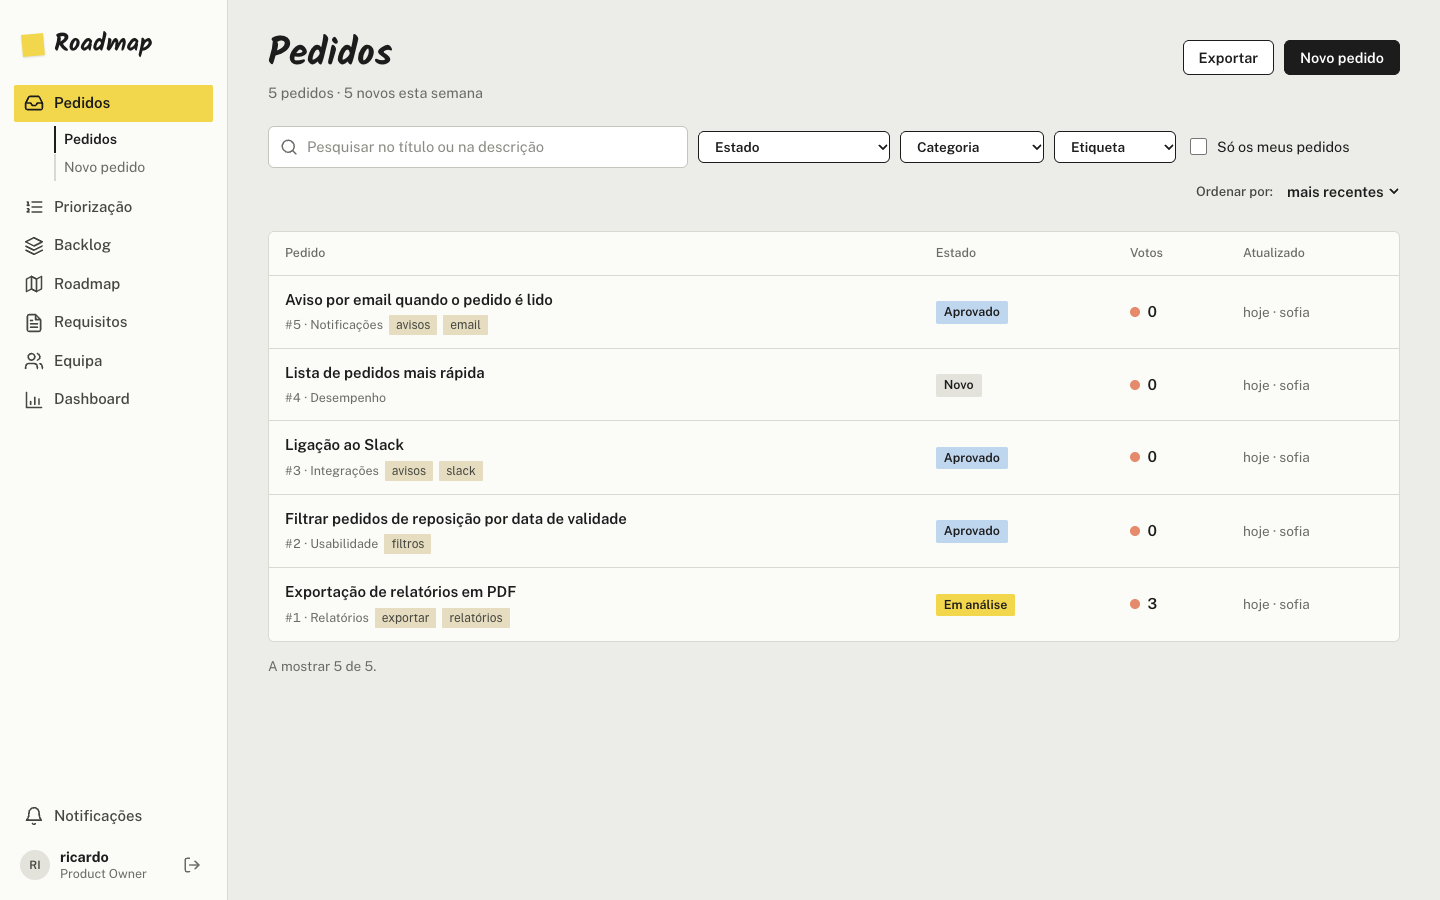
\includegraphics[width=\linewidth,height=0.7\textheight,keepaspectratio]{ecra-02-pedidos.png}
  \end{columns}
\end{frame}

\fala{Tiago}
\begin{frame}{Arquitetura: um monólito modular}
  \begin{columns}[c]
    \column{0.55\textwidth}
    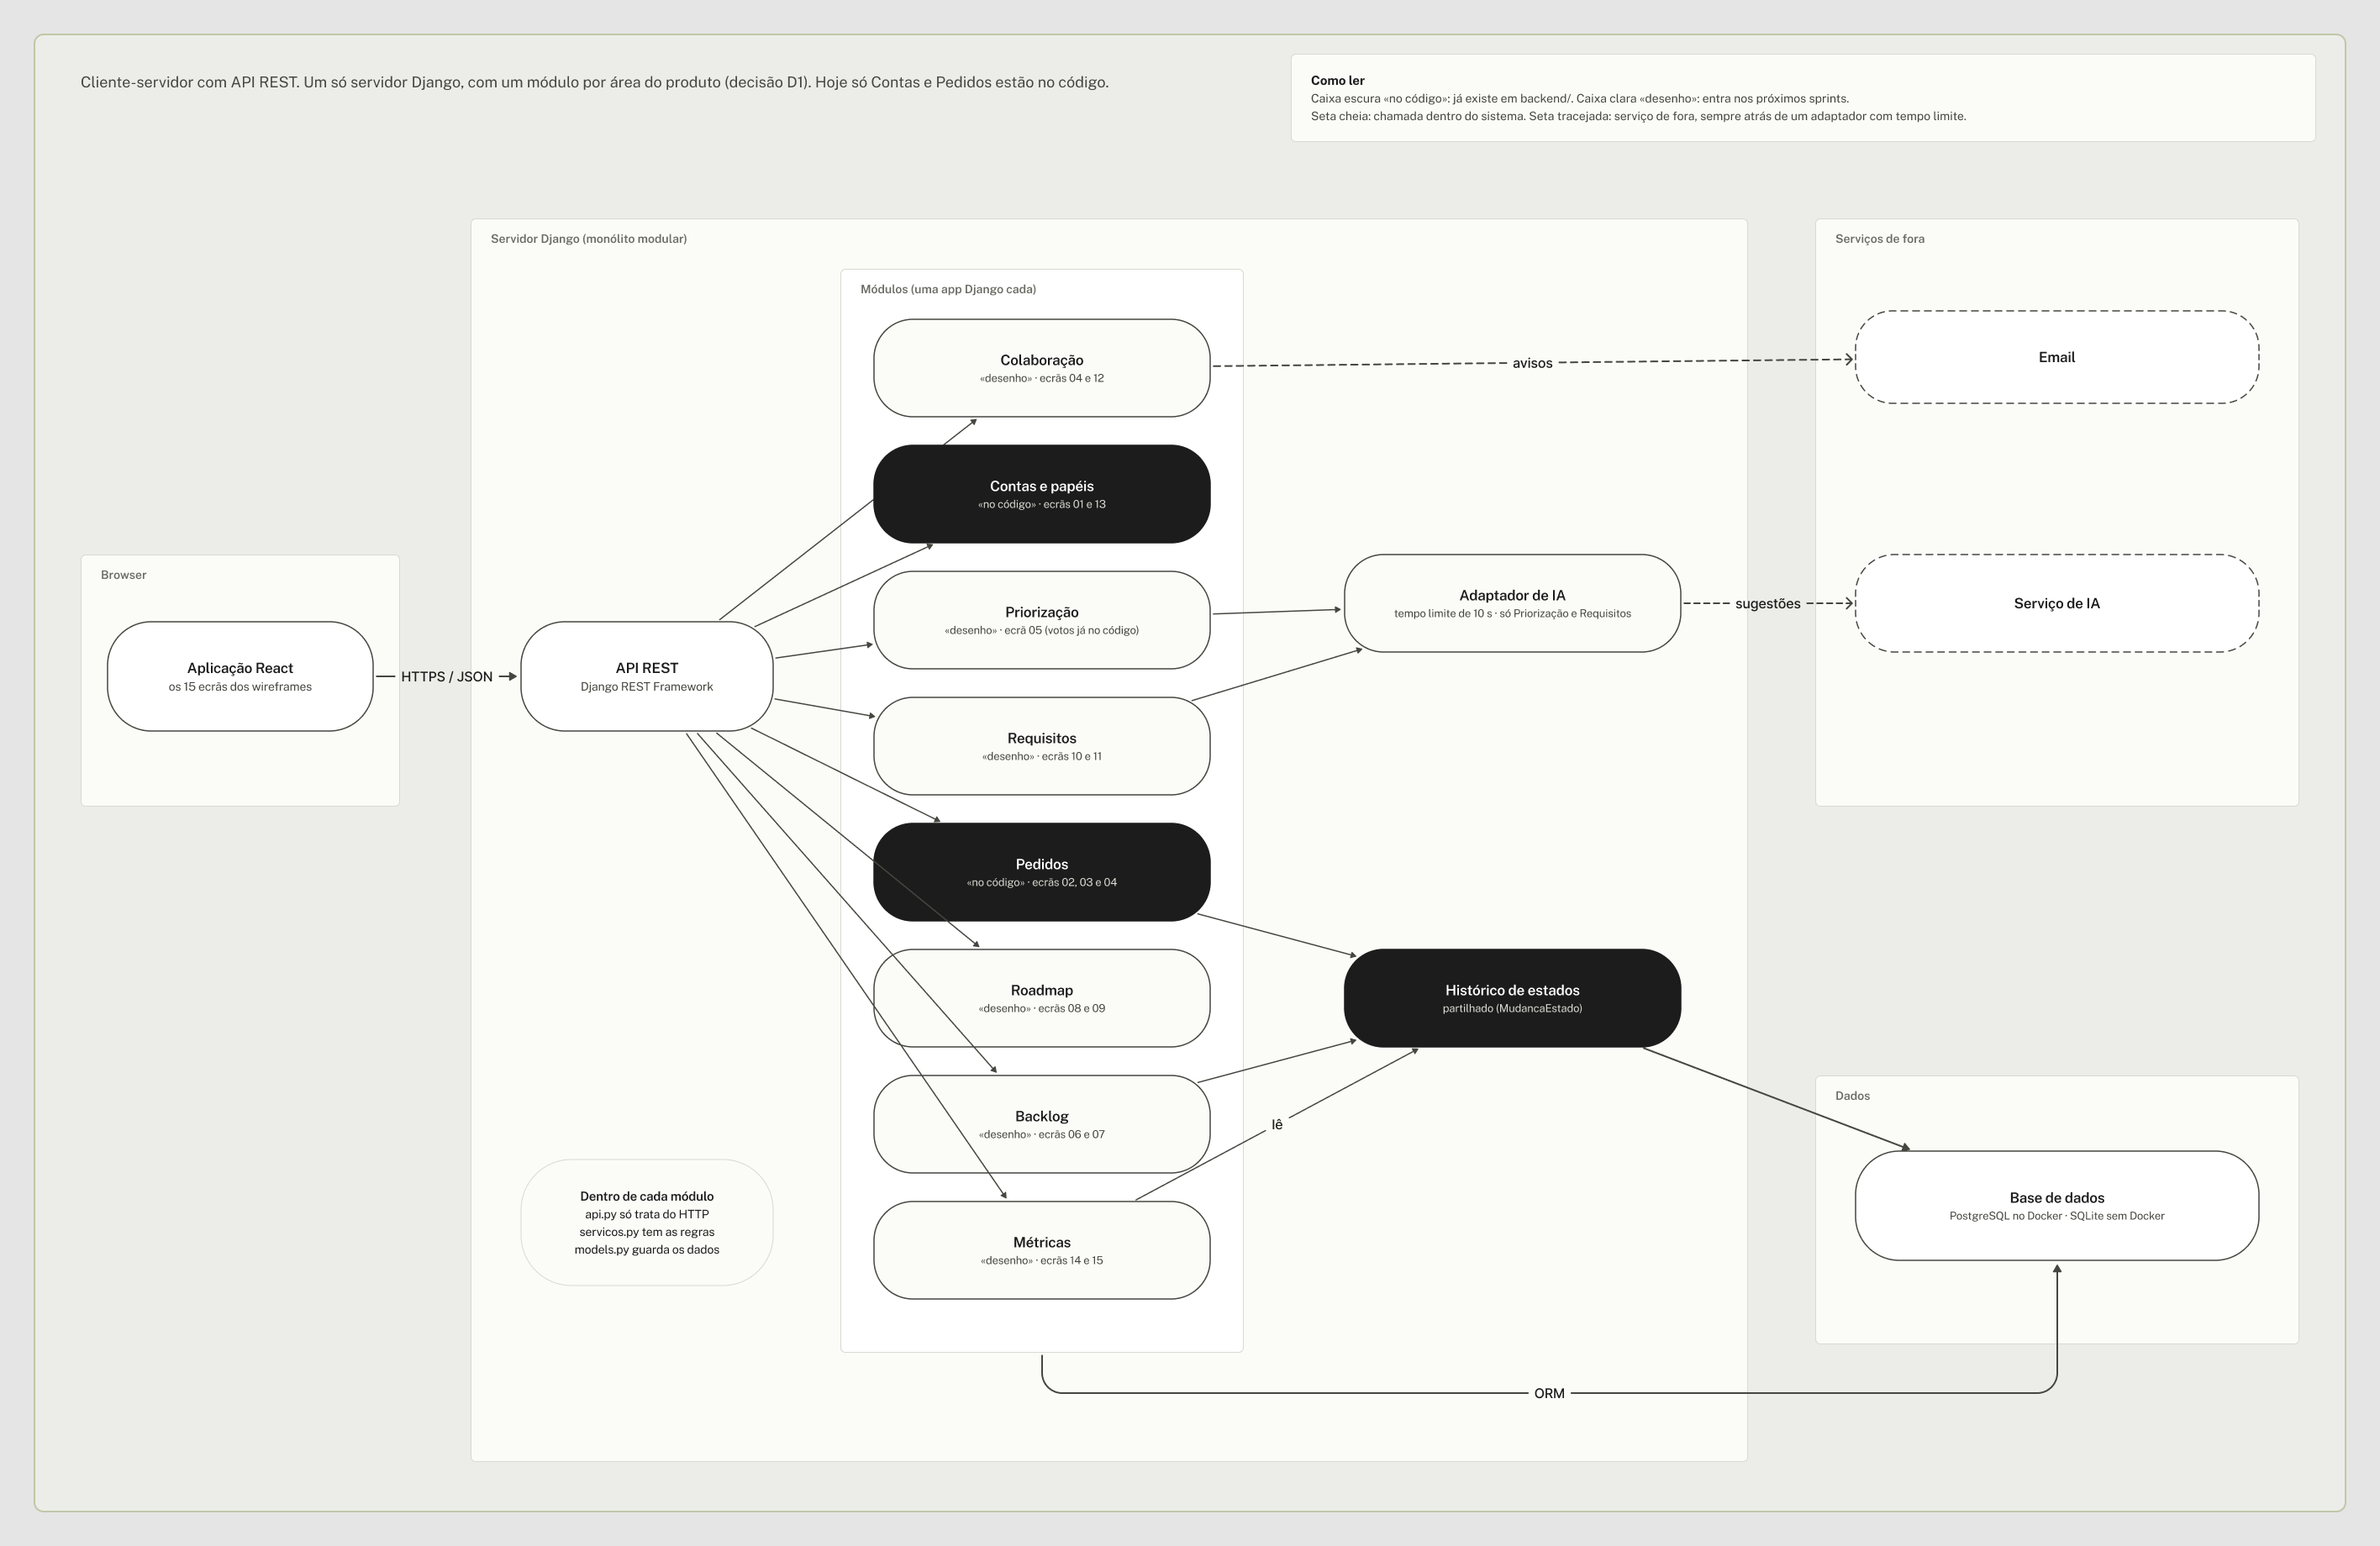
\includegraphics[width=\linewidth,height=0.72\textheight,keepaspectratio]{diagrama-01-arquitetura.png}
    \column{0.42\textwidth}
    \small
    \begin{itemize}
      \item React no browser, uma API em Django REST e PostgreSQL.
      \item Um módulo por área do produto, cada um com modelos, serviços (as regras) e API.
      \item Um só deploy, que serve uma equipa de cinco. Microserviços eram mais peças do que precisávamos.
      \item Os serviços de fora (IA e email) ficam atrás de um adaptador com tempo limite.
    \end{itemize}
  \end{columns}
\end{frame}

\begin{frame}{Modelação}
  \begin{columns}[T]
    \column{0.32\textwidth}
    \centering
    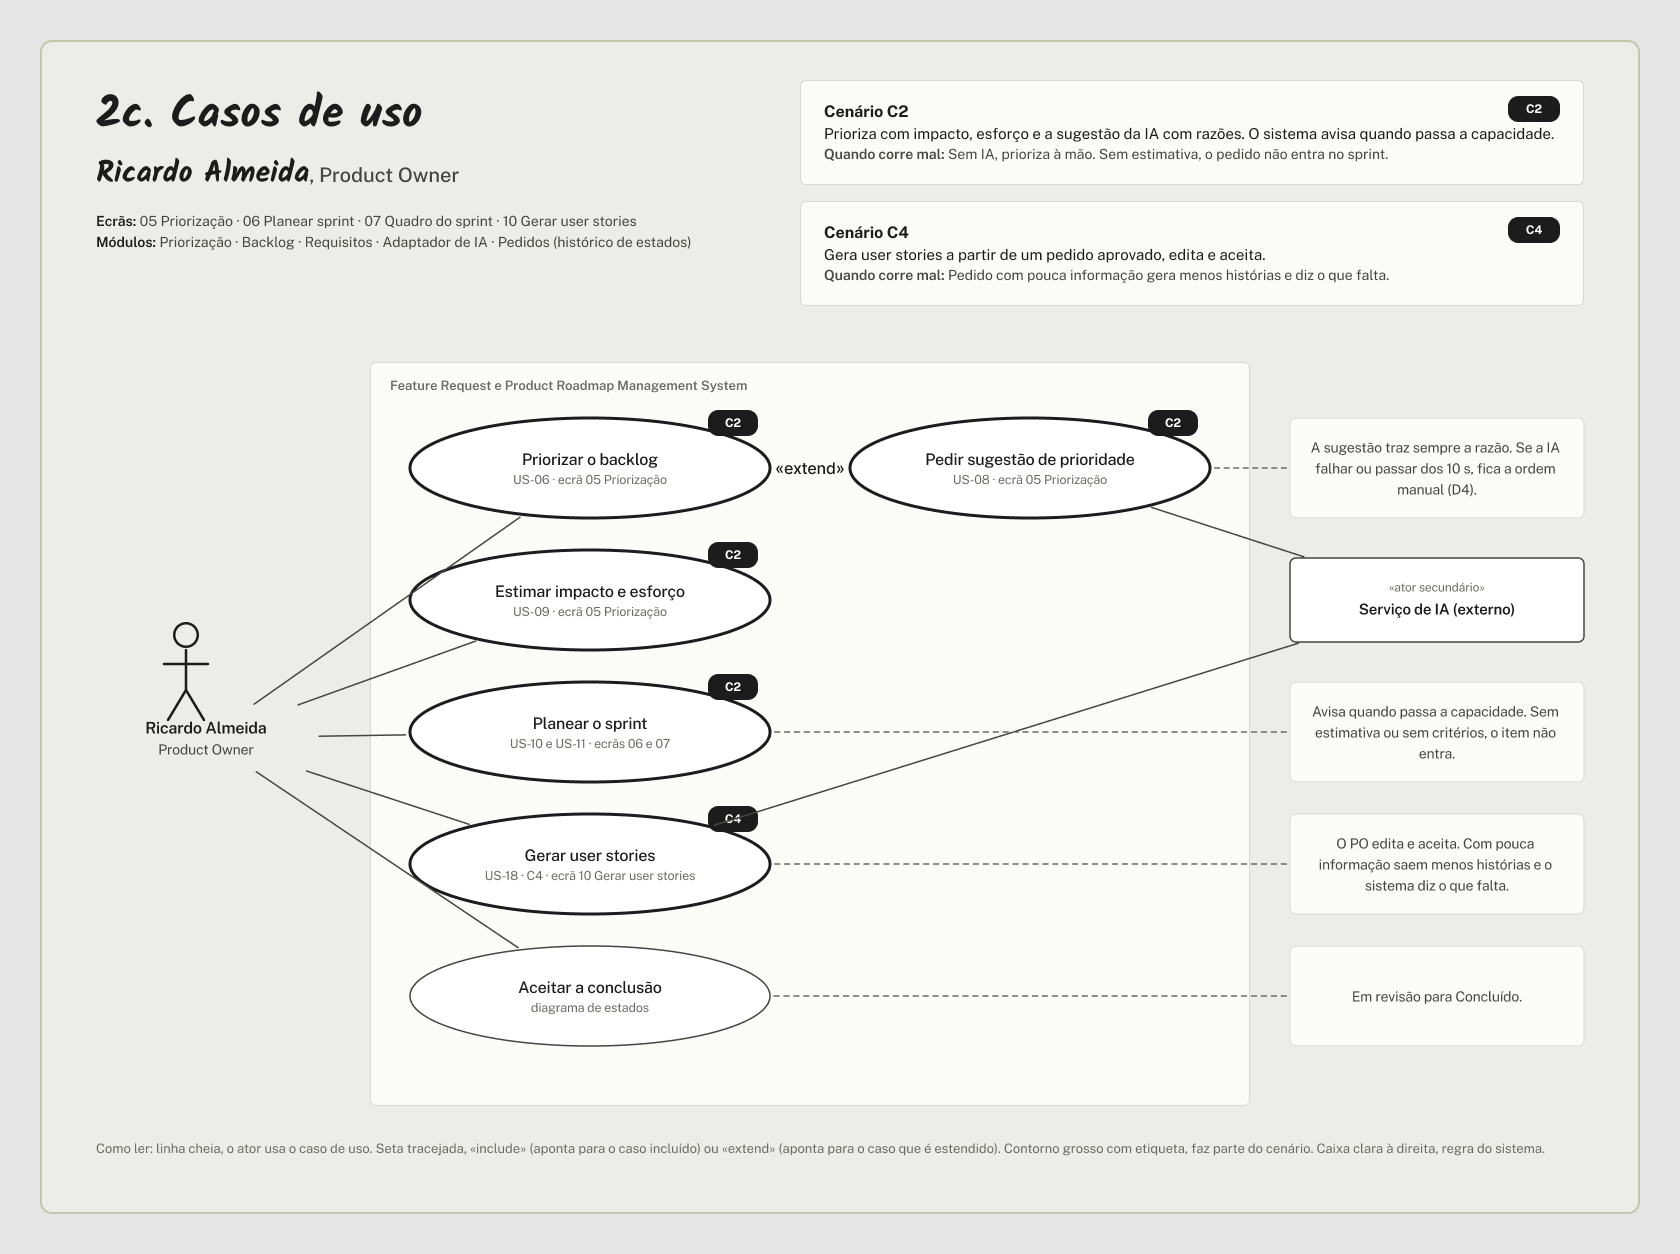
\includegraphics[width=\linewidth,height=0.5\textheight,keepaspectratio]{diagrama-02c-casos-de-uso-ricardo.png}\par
    \footnotesize Casos de uso, um diagrama por ator
    \column{0.32\textwidth}
    \centering
    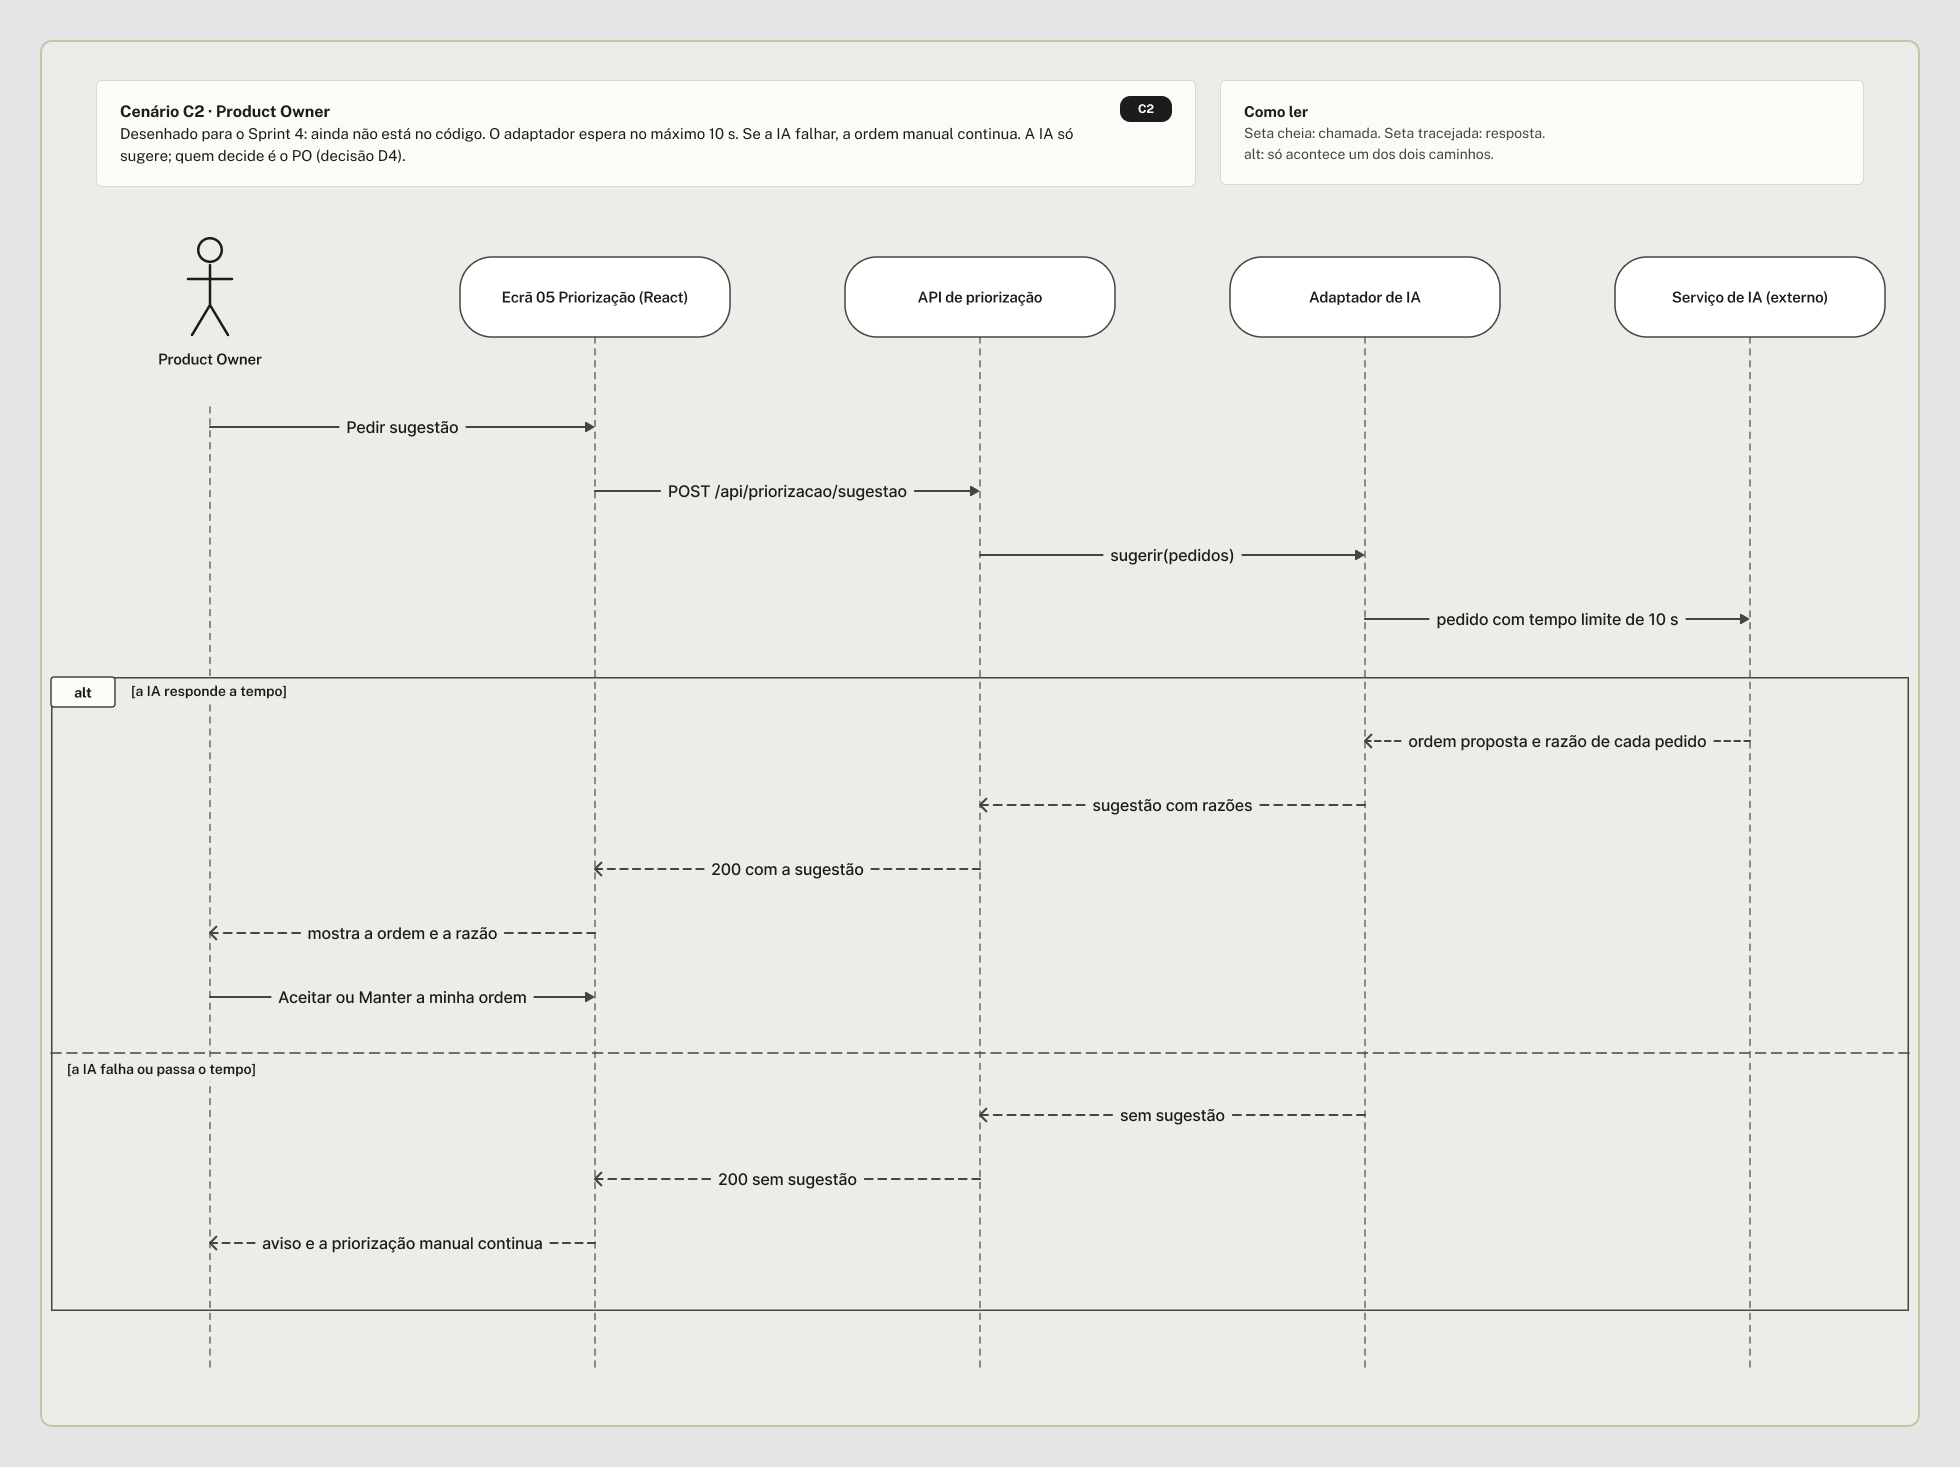
\includegraphics[width=\linewidth,height=0.5\textheight,keepaspectratio]{diagrama-03-sequencia-sugestao-ia.png}\par
    \footnotesize Sequência da sugestão de prioridade
    \column{0.32\textwidth}
    \centering
    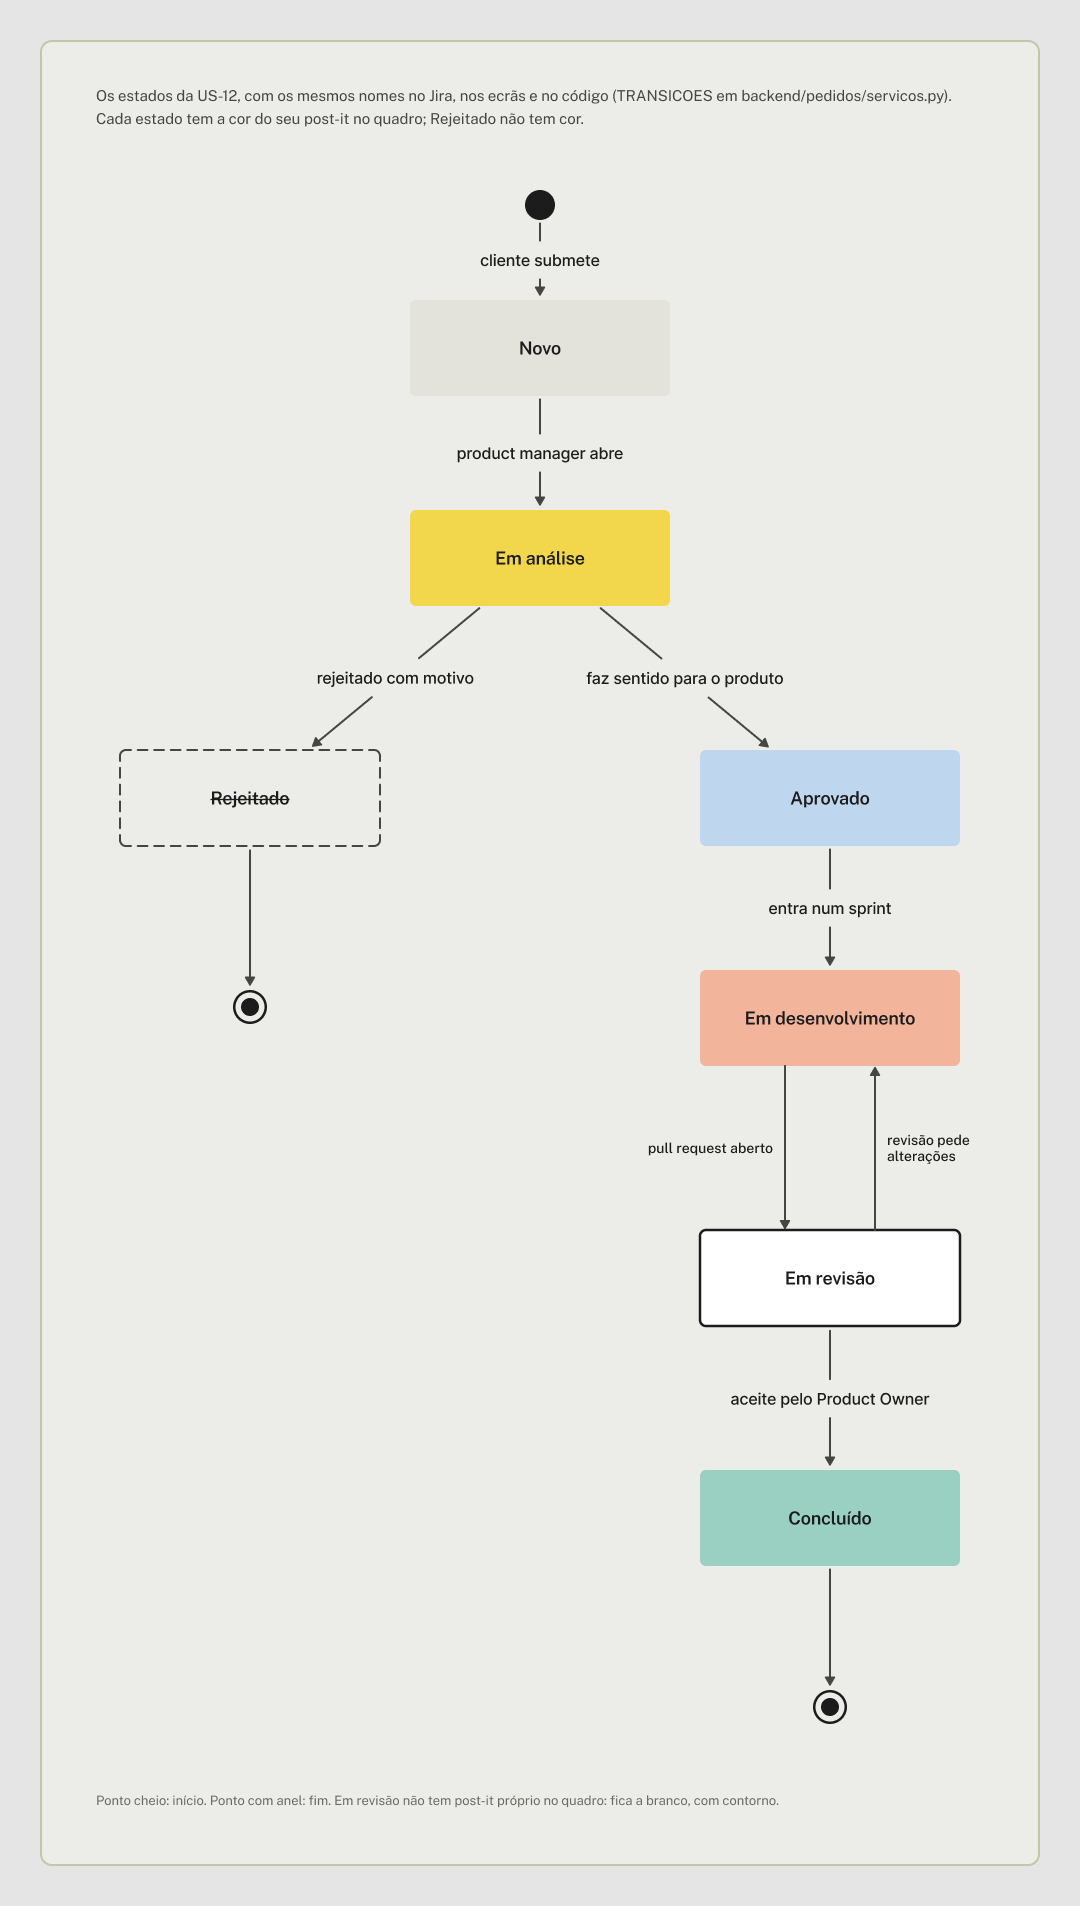
\includegraphics[width=\linewidth,height=0.5\textheight,keepaspectratio]{diagrama-06-estados-do-pedido.png}\par
    \footnotesize Estados de um pedido (US-12)
  \end{columns}
  \vspace{0.8em}
  \small Fizemos também atividades, modelo de dados e classes com uma vista por persona, como o professor pediu no Sprint 3. Os estados têm os mesmos nomes no Jira, nos diagramas, no código e nos ecrãs.
\end{frame}

\begin{frame}{O código}
  \begin{columns}[T]
    \column{0.5\textwidth}
    \small
    \begin{tabularx}{\linewidth}{@{}l X@{}}
      \toprule
      \textbf{Módulo} & \textbf{O que faz} \\
      \midrule
      \texttt{contas} & Utilizadores e papéis \\
      \texttt{pedidos} & Pedidos, votos, estados \\
      \texttt{priorizacao} & Impacto, esforço, ordem \\
      \texttt{ia} & Gemini e Claude \\
      \texttt{backlog} & Backlog, sprints, quadro \\
      \texttt{colaboracao} & Comentários, avisos \\
      \atualizar{\texttt{roadmap}} & \atualizar{Releases e milestones} \\
      \atualizar{\texttt{requisitos}} & \atualizar{User stories geradas} \\
      \atualizar{\texttt{metricas}} & \atualizar{Dashboards} \\
      \bottomrule
    \end{tabularx}
    \column{0.46\textwidth}
    \begin{itemize}
      \item Cada módulo foi feito por uma pessoa, do servidor ao ecrã, com os testes.
      \item As regras ficam nos serviços, por isso testamos as regras sem passar pela API.
      \item Quem pode fazer o quê está no servidor: o ecrã só esconde o botão.
      \item \texttt{docker compose up --build} levanta tudo.
    \end{itemize}
  \end{columns}
\end{frame}

\begin{frame}{Qualidade e versões}
  \begin{columns}[T]
    \column{0.5\textwidth}
    \textbf{Em cada push, o GitHub Actions:}
    \begin{enumerate}
      \item verifica o estilo e erros comuns (ruff);
      \item corre os testes do servidor e falha se a cobertura descer dos 90\,\%;
      \item corre os testes do front-end e faz a build.
    \end{enumerate}
    \column{0.46\textwidth}
    \textbf{Números}\par\smallskip
    \cartao{\small
      \atualizar{108} testes no servidor e \atualizar{45} no front-end\par
      Cobertura do servidor: \atualizar{96\,\%}\par
      \atualizar{98} commits, cada um com a conta de quem fez\par
      Versões: \texttt{v0.3.0}, \texttt{v0.4.0} e \atualizar{\texttt{v1.0.0}}}
  \end{columns}
  \vspace{1em}
  \small Cada sprint fecha com uma tag no Git, uma release no GitHub e a mesma versão no Jira, como o professor pediu no fim do Sprint 3.
\end{frame}

\begin{frame}{Onde usámos IA}
  \begin{columns}[T]
    \column{0.31\textwidth}
    \cartao{\textbf{Requisitos}\par\smallskip\small
      Entrevistas às personas no Character.ai, como o enunciado pede.}
    \column{0.31\textwidth}
    \cartao{\textbf{Programação}\par\smallskip\small
      Claude Code para apoiar o código, os testes e a revisão. Quem faz o commit lê, testa e responde pelo que entrega.}
    \column{0.31\textwidth}
    \cartao{\textbf{No produto}\par\smallskip\small
      Sugestão de prioridade e geração de user stories, com Gemini ou Claude, e uma regra local quando não há IA.}
  \end{columns}
  \vspace{1.2em}
  Registámos cada uso no Registo de Uso de IA (\texttt{docs/registo-ia/}), com a data, para quê e quem reviu.
\end{frame}

% ================================================================ parte 2
\section{O Sprint 5}

\fala{Rui}
\begin{frame}{Objetivo do Sprint 5}
  \begin{columns}[T]
    \column{0.52\textwidth}
    Quatro semanas, de 17 de novembro a 11 de dezembro.\par\medskip
    \cartao{\small Ligar à API os sete ecrãs que ainda usavam dados de exemplo (08 a 11 e 13 a 15), cobrir as sete áreas do enunciado e entregar a \texttt{v1.0.0}.}
    \vspace{0.8em}
    \small 14 cartões e 60 pontos no Jira (EDS-185 a EDS-198).
    \column{0.44\textwidth}
    \small
    \begin{tabularx}{\linewidth}{@{}l X@{}}
      \toprule
      \textbf{Quem} & \textbf{O quê} \\
      \midrule
      Tiago & IA, edição de pedidos, deploy \\
      Rui & Roadmap e releases \\
      Marcus & User stories e rastreabilidade \\
      João & Espaço de equipa, refactoring, manual \\
      Felipe & Métricas e carga das equipas \\
      \bottomrule
    \end{tabularx}
  \end{columns}
\end{frame}

\fala{Tiago}
\begin{frame}{A IA atrás de um só cliente}
  \begin{tikzpicture}[
      caixa/.style={draw=tinta, fill=quadro, rounded corners=2pt, minimum height=2.4em, inner xsep=0.6em, font=\small},
      seta/.style={-{Stealth[length=2mm]}, draw=tinta}]
    \node[caixa] (ecra) {Ecrãs 05 e 10};
    \node[caixa, right=1.2em of ecra] (mod) {Priorização, Requisitos};
    \node[caixa, right=1.2em of mod, fill=postit] (cli) {\texttt{ia/cliente.py}};
    \node[caixa, above right=0.4em and 1.2em of cli] (gem) {Gemini (Google)};
    \node[caixa, below right=0.4em and 1.2em of cli] (cla) {Claude (Anthropic)};
    \node[caixa, below=2.2em of mod] (loc) {Regra local};
    \draw[seta] (ecra) -- (mod);
    \draw[seta] (mod) -- (cli);
    \draw[seta] (cli) -- (gem);
    \draw[seta] (cli) -- (cla);
    \draw[seta] (mod) -- node[right, font=\footnotesize, color=cinza] {sem chave ou se falhar} (loc);
  \end{tikzpicture}
  \vspace{1em}

  \small
  \begin{itemize}
    \item A API do Claude é paga e o Gemini tem um plano gratuito, por isso ligámos os dois. Usa-se o que tiver chave.
    \item Sem chave, ou se a IA falhar, a aplicação continua com a regra local, e o ecrã diz de onde veio a sugestão.
    \item A IA só sugere: nada muda sem o Product Owner aceitar.
  \end{itemize}
\end{frame}

\begin{frame}{Pedidos: pedir, votar e acompanhar}
  \begin{columns}[c]
    \column{0.6\textwidth}
    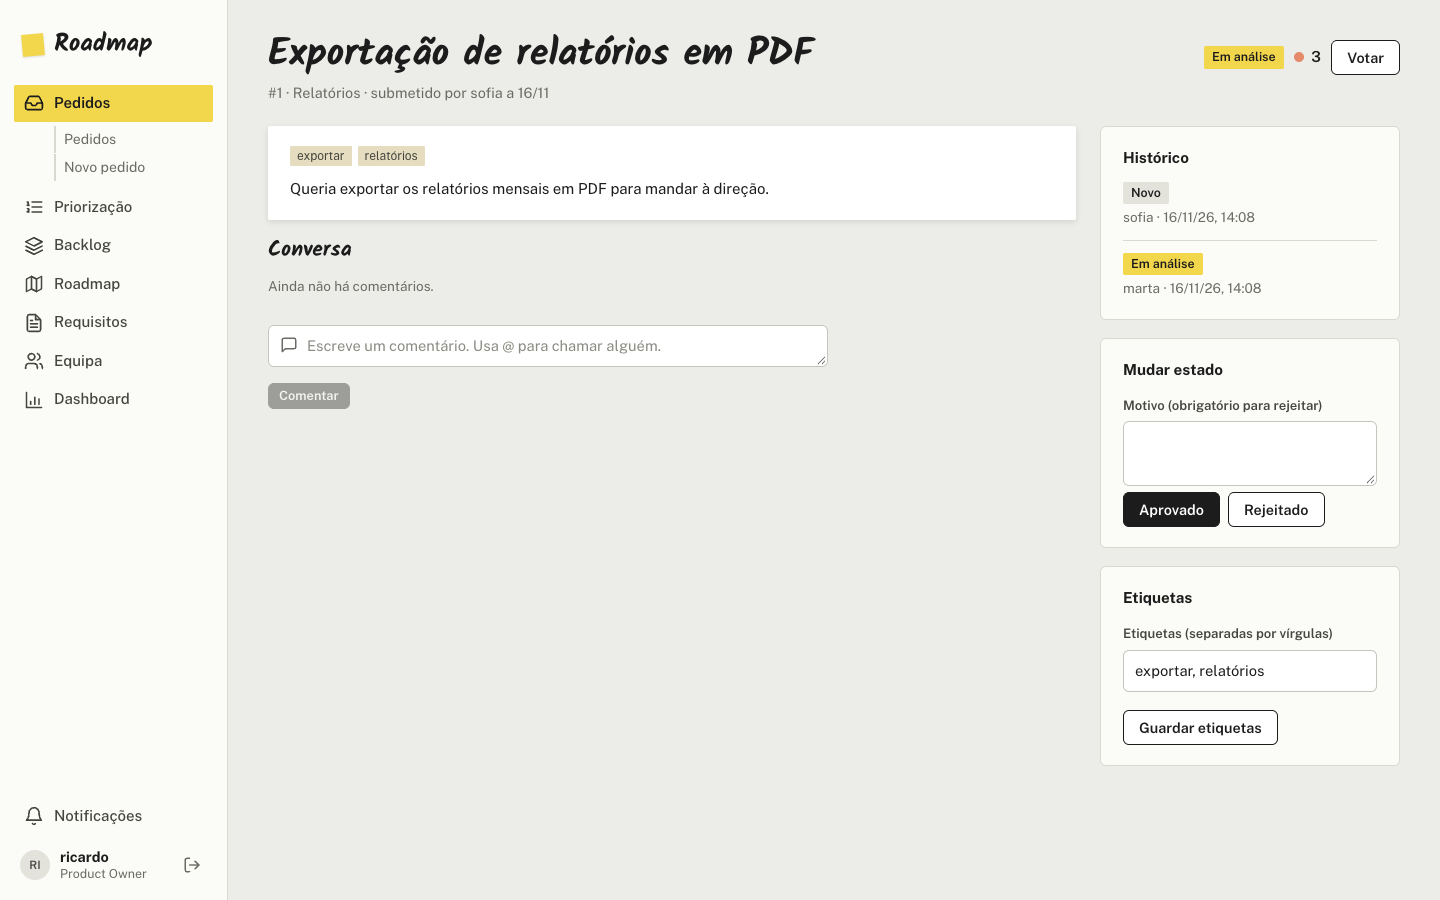
\includegraphics[width=\linewidth,height=0.75\textheight,keepaspectratio]{ecra-04-detalhe.png}
    \column{0.37\textwidth}
    \small
    \begin{itemize}
      \item Ao escrever um pedido, o sistema avisa se já há um parecido, para votar nele em vez de o repetir.
      \item Cada mudança de estado fica no histórico, com quem e quando.
      \item \atualizar{Um pedido pode ser editado, e cada edição guarda uma versão.}
    \end{itemize}
  \end{columns}
\end{frame}

\fala{Marcus}
\begin{frame}{Priorizar com ajuda da IA}
  \begin{columns}[c]
    \column{0.62\textwidth}
    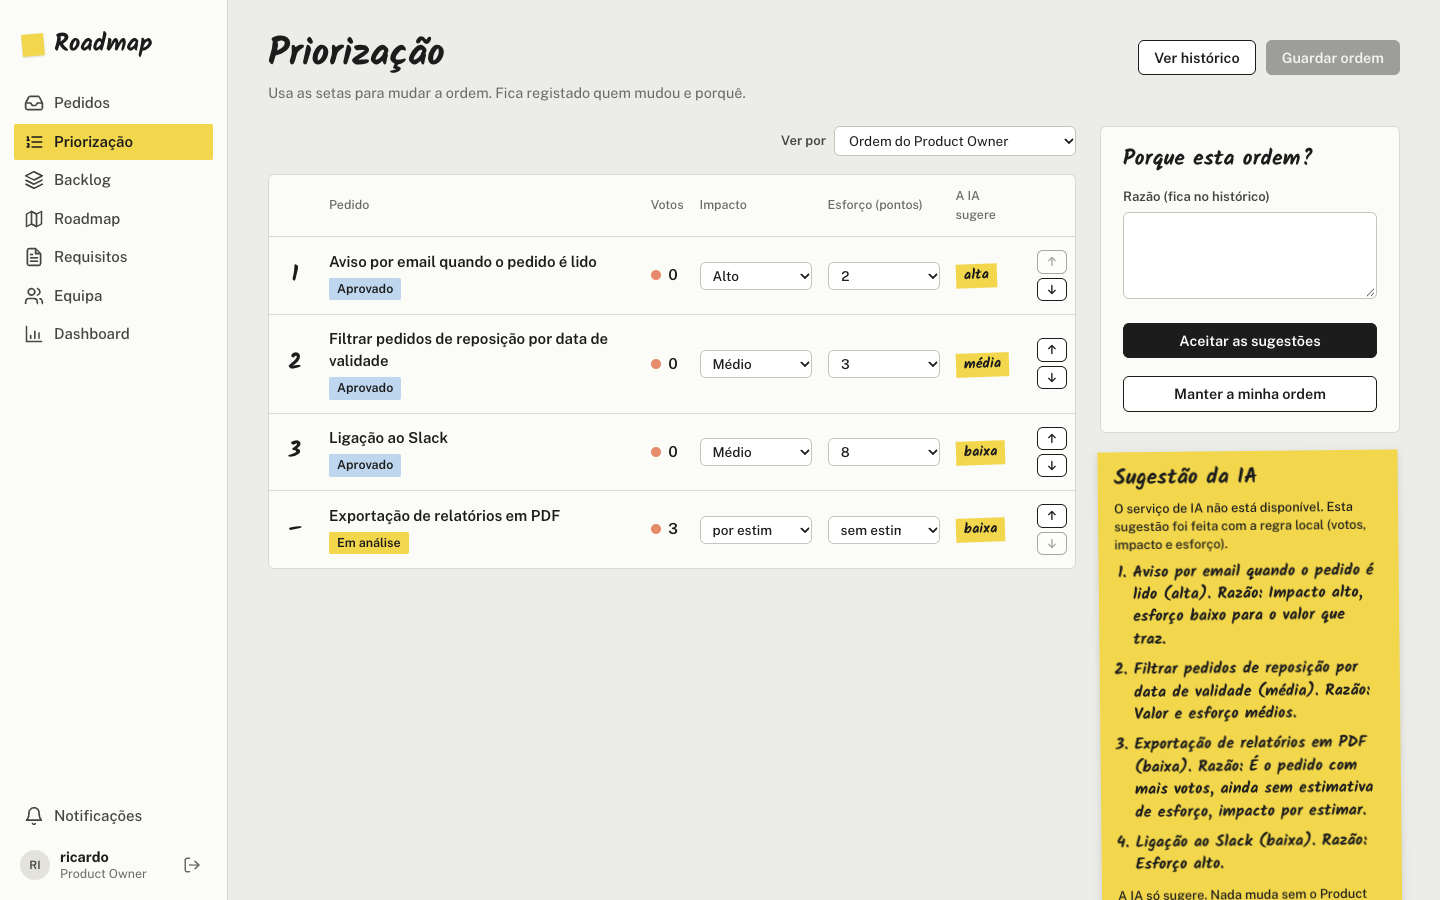
\includegraphics[width=\linewidth,height=0.75\textheight,keepaspectratio]{ecra-05-priorizacao.png}
    \column{0.35\textwidth}
    \small
    \begin{itemize}
      \item O Product Owner estima impacto e esforço e define a ordem, com a razão.
      \item A sugestão diz porquê para cada pedido.
      \item O aviso de capacidade mostra o que já não cabe no sprint.
    \end{itemize}
  \end{columns}
\end{frame}

\fala{Rui}
\begin{frame}{Backlog, sprint e roadmap}
  \begin{columns}[c]
    \column{0.6\textwidth}
    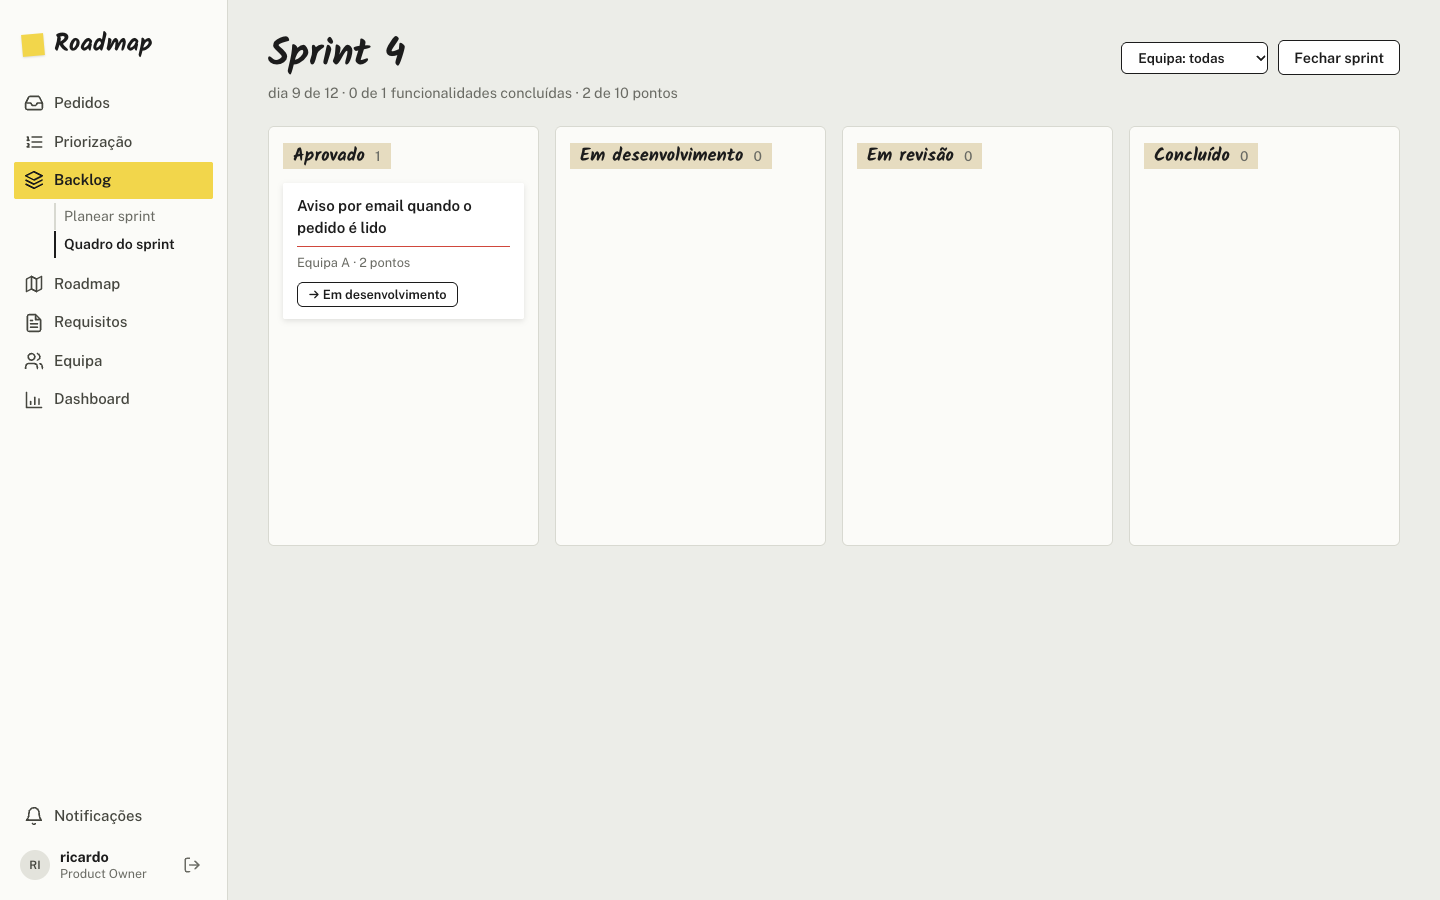
\includegraphics[width=\linewidth,height=0.75\textheight,keepaspectratio]{ecra-07-quadro.png}
    \column{0.37\textwidth}
    \small
    \begin{itemize}
      \item Só entra no sprint o que tem estimativa; o que não acaba volta ao backlog.
      \item O quadro tem uma coluna por estado e filtra por equipa.
      \item \atualizar{O roadmap mostra as releases por mês, os milestones e as dependências, e avisa quando uma release está em risco.}
    \end{itemize}
  \end{columns}
  % ATUALIZAR: trocar a imagem por uma captura do ecrã 08 (Roadmap) ligado à API.
\end{frame}

\fala{Marcus}
\begin{frame}{Requisitos: gerar user stories}
  \begin{itemize}
    \item \atualizar{A partir de um pedido aprovado, o sistema propõe user stories com critérios de aceitação, com a IA ou com um modelo local.}
    \item \atualizar{O Product Owner revê, edita e aceita; só as aceites ficam guardadas.}
    \item \atualizar{A rastreabilidade liga pedido, user story, item do sprint e release, e marca o que está por ligar.}
  \end{itemize}
  % ATUALIZAR: pôr aqui as capturas dos ecrãs 10 e 11 ligados à API.
\end{frame}

\fala{João}
\begin{frame}{Colaborar}
  \begin{columns}[c]
    \column{0.6\textwidth}
    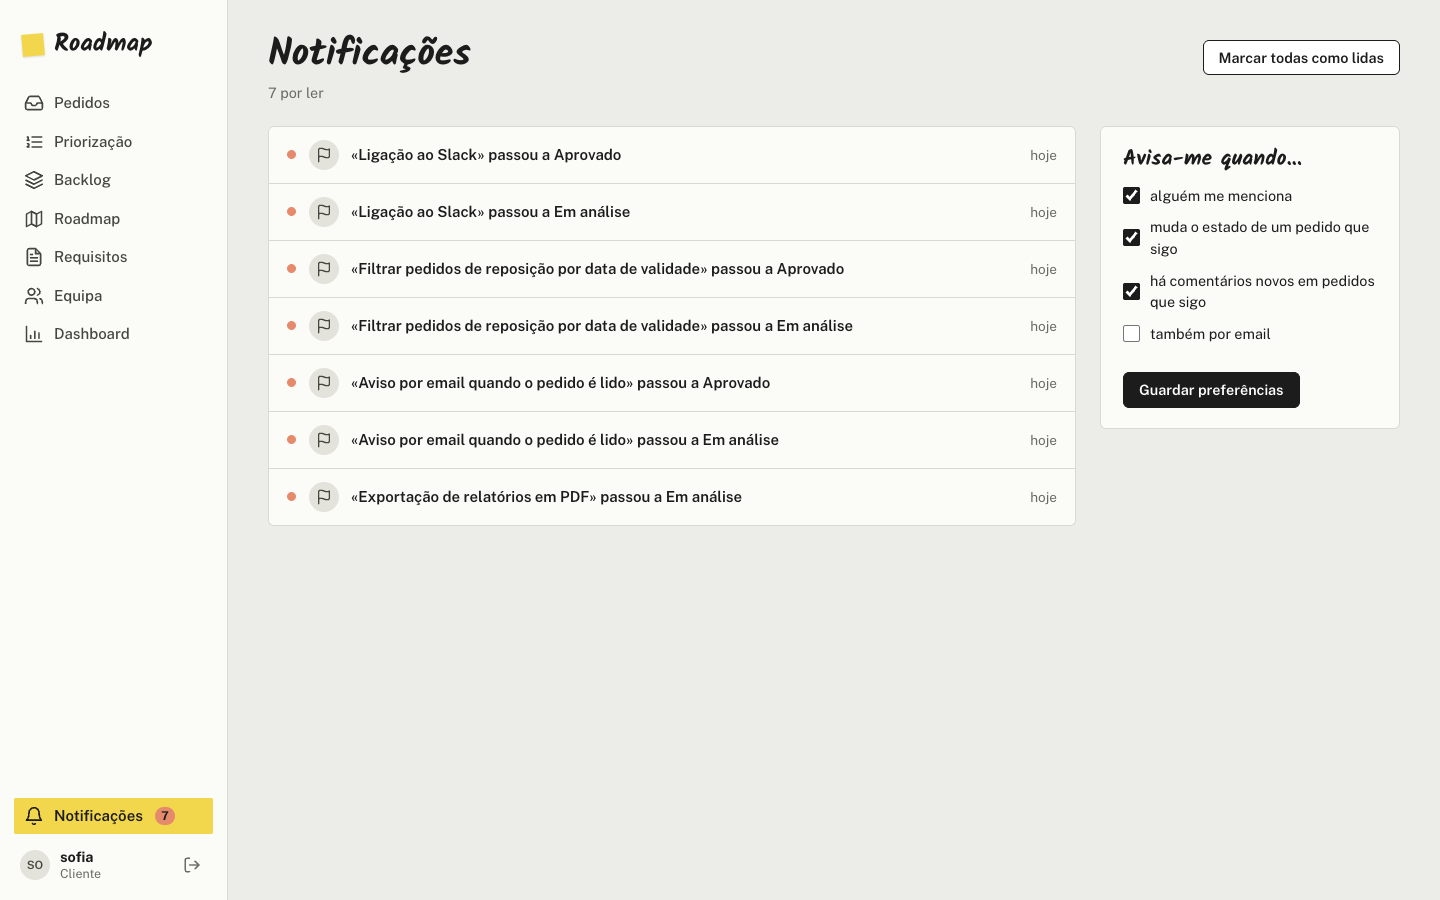
\includegraphics[width=\linewidth,height=0.75\textheight,keepaspectratio]{ecra-12-notificacoes.png}
    \column{0.37\textwidth}
    \small
    \begin{itemize}
      \item Comentários com menções (@sofia) em cada pedido.
      \item Quem pediu, votou ou comentou é avisado quando o estado muda.
      \item \atualizar{Cada equipa tem o seu espaço: membros, pedidos, sprint e conversa.}
    \end{itemize}
  \end{columns}
\end{frame}

\fala{Felipe}
\begin{frame}{Dashboards e métricas}
  \begin{itemize}
    \item \atualizar{Pedidos submetidos, aprovados e rejeitados por mês.}
    \item \atualizar{Funcionalidades por release e progresso do roadmap.}
    \item \atualizar{Lead time (de Novo a Concluído) e cycle time (de Em desenvolvimento a Concluído), calculados a partir do histórico de estados.}
    \item \atualizar{Carga de cada equipa, com aviso quando passa a capacidade.}
  \end{itemize}
  % ATUALIZAR: pôr aqui as capturas dos ecrãs 14 e 15 ligados à API.
\end{frame}

\fala{João}
\begin{frame}{Refactoring}
  \small
  \begin{tabularx}{\textwidth}{@{}X X X@{}}
    \toprule
    \textbf{Antes} & \textbf{Depois} & \textbf{Porquê} \\
    \midrule
    A ligação ao Claude estava dentro da priorização & Uma pasta \texttt{ia/} com um cliente e um ficheiro por serviço & A geração de user stories também precisa de IA; trocar de serviço passa a ser mudar uma variável \\
    \atualizar{(por preencher)} & \atualizar{(por preencher)} & \atualizar{(por preencher)} \\
    \atualizar{(por preencher)} & \atualizar{(por preencher)} & \atualizar{(por preencher)} \\
    \bottomrule
  \end{tabularx}
  \vspace{0.8em}

  Cada refactoring teve os testes a passar antes e depois (cartão EDS-192).
\end{frame}

\fala{Tiago}
\begin{frame}{Do commit à versão publicada}
  \begin{tikzpicture}[
      passo/.style={draw=tinta, fill=quadro, rounded corners=2pt, minimum height=2.6em, text width=6.2em, align=center, font=\small},
      seta/.style={-{Stealth[length=2mm]}, draw=tinta}]
    \node[passo] (a) {Commit e push na \texttt{main}};
    \node[passo, right=1.4em of a] (b) {Ruff e testes};
    \node[passo, right=1.4em of b] (c) {Cobertura $\geq$ 90\,\%};
    \node[passo, right=1.4em of c, fill=postit] (d) {\atualizar{Imagens Docker publicadas}};
    \node[passo, right=1.4em of d] (e) {Tag e release};
    \draw[seta] (a) -- (b); \draw[seta] (b) -- (c); \draw[seta] (c) -- (d); \draw[seta] (d) -- (e);
  \end{tikzpicture}
  \vspace{1.5em}

  \begin{itemize}
    \item Se um passo falha, os seguintes não correm: nada chega à versão publicada com testes a vermelho.
    \item \atualizar{As imagens do back-end e do front-end ficam no GitHub, e quem quiser corre a versão final sem compilar.}
  \end{itemize}
\end{frame}

\fala{Rui}
\begin{frame}{O enunciado, ponto por ponto}
  \footnotesize
  \begin{tabularx}{\textwidth}{@{}X l@{}}
    \toprule
    \textbf{Pedido} & \textbf{Onde está} \\
    \midrule
    Personas, cenários e user stories & Jira (epics EDS-150 a 152) e \texttt{wiki/01-produto} \\
    Requisitos com o Character.ai & Cinco entrevistas (EDS-55), \texttt{wiki/02-requisitos} \\
    Wireframes e mockups & Figma, \texttt{docs/sprint-3/wireframes} \\
    Arquitetura justificada & \texttt{wiki/04-arquitetura}, registo de decisões \\
    Desenho e modelação & FigJam, \texttt{docs/sprint-3/modelacao} \\
    Back-end e front-end, 8 interfaces além do login & \atualizar{14 ecrãs ligados à API} \\
    Testes e integração contínua & GitHub Actions em cada push \\
    Ferramenta de IA para programar & Claude Code (EDS-12), Registo de Uso de IA \\
    Rotação de Product Owner e Scrum Master & Contrato e Jira \\
    \bottomrule
  \end{tabularx}
\end{frame}

\fala{Tiago}
\begin{frame}{O que aprendemos}
  \begin{columns}[T]
    \column{0.48\textwidth}
    \textbf{O que correu mal}
    \begin{itemize}\small
      \item No início analisámos o produto errado (o exercício do Lab03); só a 14 de outubro fechámos o produto do enunciado.
      \item Os primeiros wireframes não respondiam a tudo o que as personas pediram. Corrigimo-los no Sprint 3.
      \item Os registos das cerimónias no Jira ficaram atrasados em alguns sprints.
    \end{itemize}
    \column{0.48\textwidth}
    \textbf{O que correu bem}
    \begin{itemize}\small
      \item Ter testes e integração contínua desde o Sprint 3 deixou-nos mudar o código sem medo.
      \item Um módulo por pessoa: cada um sabe explicar a sua parte.
      \item O feedback do professor entrou no sprint seguinte (versões, testes, casos de uso por ator).
    \end{itemize}
  \end{columns}
  \vspace{0.6em}
  \small\atualizar{(Acrescentar aqui o que sair da Retrospetiva do Sprint 5, EDS-47.)}
\end{frame}

\fala{Todos}
\begin{frame}[plain]
  \vfill
  {\Huge\bfseries Obrigado.}\par\medskip
  {\large\color{cinza}Perguntas?}\par\vspace{2em}
  \small
  Código: \texttt{github.com/TiagoPereira001/UBI\_ES-PedidosERoadmap}\par
  Jira: projeto EDS\quad·\quad Documentação: pasta \texttt{wiki/} do repositório
  \vfill
\end{frame}

\end{document}
